\section{Binary evolution and Dynamo model}
%------------------------------------------------------------------
\begin{table*}
\centering
\begin{tabular}{c c c c c c c c}
\hline
\hline
  Binary & 
$Md[M_{\odot}]$&$Rd[R_{\odot}]$&$Mg[M_{\odot}]$&q&$P_{orb}[d]$&$P_{long}[d]$&$P_{long}/P_{orb}$\\
\hline
    U Cep   & $3.22\pm 0.143$ & $7.045\pm 0.279$ & $4.938\pm 0.532$ & $0.652$ & $3.38\pm (0.05)$ & $515-26663$&152-7889\\
   
   UX Mon   & $3.9\pm 0.29$ & $9.8\pm 0.003$ & $3.38\pm 0.4$ & $1.15$ & $5.90\pm 0.005$ & no$^{(1)}$&- \\
   
   DQ Vel   & $2.2\pm 0.2$ & $8.4\pm 0.2$ &$7.3\pm 0.3$& $0.31$ &$6.08337\pm 0.00013$&$189$&31.1 \\
   
   V448 Cyg & $13.7\pm 0.7$ & $16.3\pm 0.3$ & $24.7\pm 0.7$ & $0.55$ & $6.52\pm (0.05)$ & $no$&-\\
   
   CX Dra  & $1.7\pm$ (0.5)& $13.25\pm (0.05)$ & $7.3\pm (0.5)$& $0.23$&$6.95957\pm 0.000043$&yes&- \\
   
   TT Hya  & $0.63\pm (0.05)$ & $4.3\pm (0.5)$ & $2.77\pm (0.05)$ & $0.23$ & $6.95\pm (0.05)$ & $?$&-\\
   
   iDPV    & $1.9\pm 0.2$ & $8.9\pm 0.3$ & $9.1\pm 0.5$ & $0.21$ &$7.241\pm (0.005)$ &$172$&23.8 \\
   
   V393 Sco& $2.0\pm 0.2$ & $9.4\pm 0.50$ & $7.8\pm 0.30$ & $0.25$ & $7.71259\pm (0.00005)$ & $253$&32.8 \\
   
   LP Ara  & $3.0\pm (0.5)$ &$11.6\pm (0.5)$ &$9.8\pm (0.5)$ &$0.30$ &$8.53295\pm(0.000005)$ & $273$&32 \\
   
   V360 Lac& $1.2\pm 0.05$ & $8.8\pm (0.5)$ & $7.45\pm 0.3$ & $0.16$ & $10.085449\pm 0.000078$ & $322.2$&31.9 \\
   
   AU Mon  & $1.20\pm 0.2$ & $10.1\pm0.5$ & $7.0\pm 0.3$ & $0.17$ & $11.1130374\pm 0.0000001$ & $421$ &37.9 \\
   
  BR CMi  & $0.137^{+0.0017}_{-0.0026}$&$5.49^{+0.22}_{-0.37}$&$2.31^{+0.29}_{-0.43}$&$0.06$&$12.919\pm 0.000015$&$no$&- \\
   
   $\beta$ Lyr &$2.97\pm 0.2$&$15.2\pm 0.2$&$13.16\pm 0.3$&$0.23$&$12.941\pm 0.002$&$282.4$&21.8\\

HD170582& $1.9\pm 0.1$ & $15.6\pm 0.2$ &$9.0\pm 0.2$& $0.21$&$16.87177\pm 0.002084$&$537$&31.8\\

RX Cas& $1.8\pm 0.4$ & $23.5\pm 1.2$ & $5.8\pm 0.5$ & $0.32$ & $32.31211\pm (0.00005)$ & $516.1$&16\\

V495 Cen& $0.91\pm 0.2$ & $19.3\pm 0.5$ & $5.76 \pm 0.3$ & $0.17$ & $33.492\pm 0.002$ & $1283$&38.3\\

SX Cas& $1.5\pm 0.4$ & $23.5\pm 1.3$ & $5.1\pm 0.4$ & $0.29$ & $36.56\pm (0.05)$ & $?$&-\\
\hline
\end{tabular}
\caption{The table includes both donor and gainer masses, donor radius, ratio $q=M_{d}/M_{g}$
, orbital period, the available information on the presence of a long period and the ratio $P_{long}/P_{orb}$ as well as the error for each parameter where the number in () means that we are estimating the error affecting only the last digit.}
\label{table:sample}
\end{table*}


%------------------------------------------------------------------
In this section, we compare the systems parameters listed in table \ref{table:sample} with those predicted by binary evolution models which include epochs of non-conservative evolution. We inspected all the 561 conservative and non-conservative evolutionary tracks proposed by \citet{vanrensbergen2008, vanrensbergen2011} that are available at the Center Done\'es Stellaires (CDS) in order to find the model that describes the best each system in our sample. We performed a multiparametric fit by doing a $\chi^{2}$ minimization following the work by \citet{mennickent2012}, given by
\begin{eqnarray}
\chi^{2}_{i,j}=\left(\frac{1}{N}\right)\sum_{k}w_{k}\left[\frac{(S_{i,j,k}-O_{k})}{O_{k}}\right]^{2},
\end{eqnarray}
here $N$ is the number of observations (7), $S_{i,j,k}$ is the synthetic model where $i$ indicates the model, $j$ indicates the time $t_{j}$ and k indicates the stellar or orbital parameter, $O_{k}$ are the observed stellar parameters we are using to perform our fit, which are: mass, radii, luminosities and orbital period. The quantity $w_{k}$ is the statistical wight of the parameter $O_{k}$ which is calculated as
\begin{eqnarray}
w_{k}=\sqrt{\frac{O_{k}}{\epsilon O_{k}}},
\end{eqnarray} 
where $\epsilon O_{k}$ is the error associated to the parameter $O_{k}$. The model with the minimum $\chi^{2}$ will correspond to the model with the best evolutionary system for the corresponding system and the absolute minimum $\chi^{2}$ will identifies the theoretical stellar parameters as well as the age of the system.

\subsection{Fitting observed systems to evolutionary tracks}
%-------------------------------------------
\begin{table*}
\centering
\begin{tabular}{c c c c c c c c}
\hline
\hline
    Binary & 
$Md[M_{\odot}]_{model}$&$Rd[R_{\odot}]_{model}$&$Mg[M_{\odot}]_{model}$&$R_{g}[R_{\odot}]_{model}$&$P_{orb}[d]_{model}$&$\chi^{2}_{min}$\\
    \hline
   
   DQ Vel   & $2.36$ & $8.64$ &$7.23$& $3.62$&$6.05$&$0.0058$\\
   
   iDPV    & $1.95$ & $9.09$ & $9.25$& $4.82$ &$7.24$ &$0.0215$\\
   
   V393 Sco& $2.11$ & $9.55$ & $7.49$& $3.79$& $7.71$ & $0.0163$\\
   
   LP Ara  & $2.36$ &$10.79$ &$8.83$& $4.79$&$8.51$ & $0.0465$\\
   
   V360 Lac& $1.16$ & $9.45$ & $7.24$&$6.74$ & $10.14$ & $0.0130$\\
   
   AU Mon  & $1.48$ & $11.11$ & $5.52$& $4.74$& $11.13$ & $0.1077$ \\
   
   $\beta$ Lyr &$2.25$&$14.36$&$13.31$& $6.02$&$12.95$&$0.0297$\\

HD170582& $2.01$ & $16.28$ &$9.24$ & $6.15$& $16.78$&$0.0226$\\

RX Cas& $1.72$ & $24.04$ & $6.69$ & $3.21$& $32.48$ & $0.0585$\\

V495 Cen& $1.42$ & $21.64$ & $6.49$ & $3.49$& $31.98$ & $0.179$\\

SX Cas& $1.34$ & $23.05$ & $6.57$ &$3.26$ & $36.35$ & $0.0679$&\\
\hline
\end{tabular}
\caption{The table shows each parameter predicted by van Rensbergen binary evolution models of each binary component for every system. Also is shown the minimum $\chi^{2}$ obtained for every system.}
\label{table:prediction}
\end{table*}
%-------------------------------------------
\indent We have found a good model match for 11 out of 17 systems in our sample. All the parameters predicted by the \citet{vanrensbergen2008, vanrensbergen2011} binary evolution models are listed in table \ref{table:prediction}. We can note that the models predicts in a good way the eleven well fitted systems. For the donor components of each system the deviation between model and observations is between $\sim 2\% - 56\%$ for the mass, for the radius this differece is between $\sim 1\% - 12\%$. On the other hand, for the gainer component of the systems there is a difference between prediction and observations of about $\sim 0.95\% - 21.1\%$ for the mass and $\sim 0.61\% - 28.43\%$ for the radius. For the orbital period $P_{orb}$ the deviation between model prediction and observations is between $0\% - 5\%$.


\begin{figure}[h!]
  \resizebox{\hsize}{!}{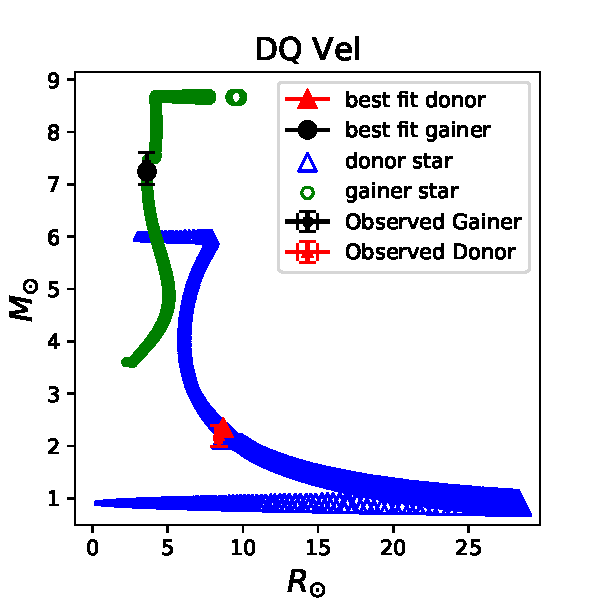
\includegraphics{dqvelfit.pdf}}
  \caption{Best fit of van Rensbergen binary evolution model for the system DQ Velorum with a $\chi^{2}\sim 0.021$. The figure shows the evolutionary track of the mass as a function of radius for both donor (blue) and gainer (green) star of the as well as the predicted current state of each component and the observed state of the system. Also the figure shows the predicted state of both components of the system with non-error bars black dot (gainer) and red triangle (donor) as well as the observed state of the each component marked with error bars black dot (gainer) and red dot (donor). The fit has the following ratios between observed and predicted parameters: $M_{d, obs}/M_{d, model}=0.94$, $M_{g, obs}/M_{g, model}=1.007$, $R_{d, obs}/R_{d, model}=0.97$, $R_{d, obs}/R_{d, model}=0.99$, $P_{orb, obs}/P_{orb, model}=0.99$.}
  \label{dqvel_fit}
\end{figure}



\subsection{The dynamo model}

We focused this work in the model proposed by \citet{schleicher2017}, using the relation between long period and orbital period \citep{soon1993, baliunas1996}
\begin{eqnarray}
P_{long}=D^{\alpha}P_{rot},
\end{eqnarray}
with $D$ the dynamo number, $P_{long}$ the activity cycle of the star and $P_{rot}$ the rotational period of the star. As DPVs are close binaries, we are able to assume that the system is tidally locked \citep{zahn1989, zahnbouchet1989}, making $P_{rot}$ equal to the binary period. $\alpha$ is a power law index that depends on the activity level of the star \citep{dube2013} and it is normally between $\sim \frac{1}{3}$ and $\sim \frac{5}{6}$. \citet{schleicher2017} found a value of $\alpha=0.31$ which yields to a good agreement of the observational data with the average population.  $D$ can be related to the rossby number by the relation $D=Ro^{-2}$, where $Ro=P_{rot}/\tau_{c}$ is defined as the ratio between the stellar rotational period $P_{rot}$ and the convective turnover time, $\tau_{c}=2H_{p}/v_{c}$. Following \citet{soker2000}, Rossby number $Ro$ can be written as
\begin{eqnarray}
Ro=9\left(\frac{v_{c}}{10\textnormal{km/s}}\right)\left(\frac{H_{p}}{40R_{\odot}}\right)^{-1}\left(\frac{\omega}{0.1\omega_{Kep}}\right)^{-1}\left(\frac{P_{Kep}}{yr}\right),
\end{eqnarray}
where $v_{c}$ and $H_{p}$ are the convective velocity and pressure scale height of the star, repectively. $\omega$ is the angular velocity, $\omega_{Kep}$ and $P_{Kep}$ are the Keplerian angular velocity and orbital period, respectively. In order to perform our analysis we follow the derivation proposed by \citet{schleicher2017} where they studied the dependance of the dynamo number on the stellar parameters by using mixing length theory, finding the following expresion
\begin{eqnarray}
P_{long}=P_{rot}\left(11.5\left(\frac{2\sqrt{2}}{15}\right)^{1/3}\frac{R_{\odot}}{km\, s^{-1}yr}\right)^{-2\alpha}\\ \nonumber
\times\left(\frac{L_{2}^{2/3}R_{2}^{2/3}}{M_{2}^{2/3}}\left(\frac{l_{m}}{H_{p}}\right)^{-4/3}\left(\frac{P_{kep}}{\epsilon_{H}R_{2}}\right)^{2}\right)^{-\alpha}.
\end{eqnarray}
with $l_{m}$ the mixing length.


%-------------------------------------------

\subsection{Typical evolution of a representative system.}

\begin{figure*}[h!]
  \resizebox{\hsize}{!}{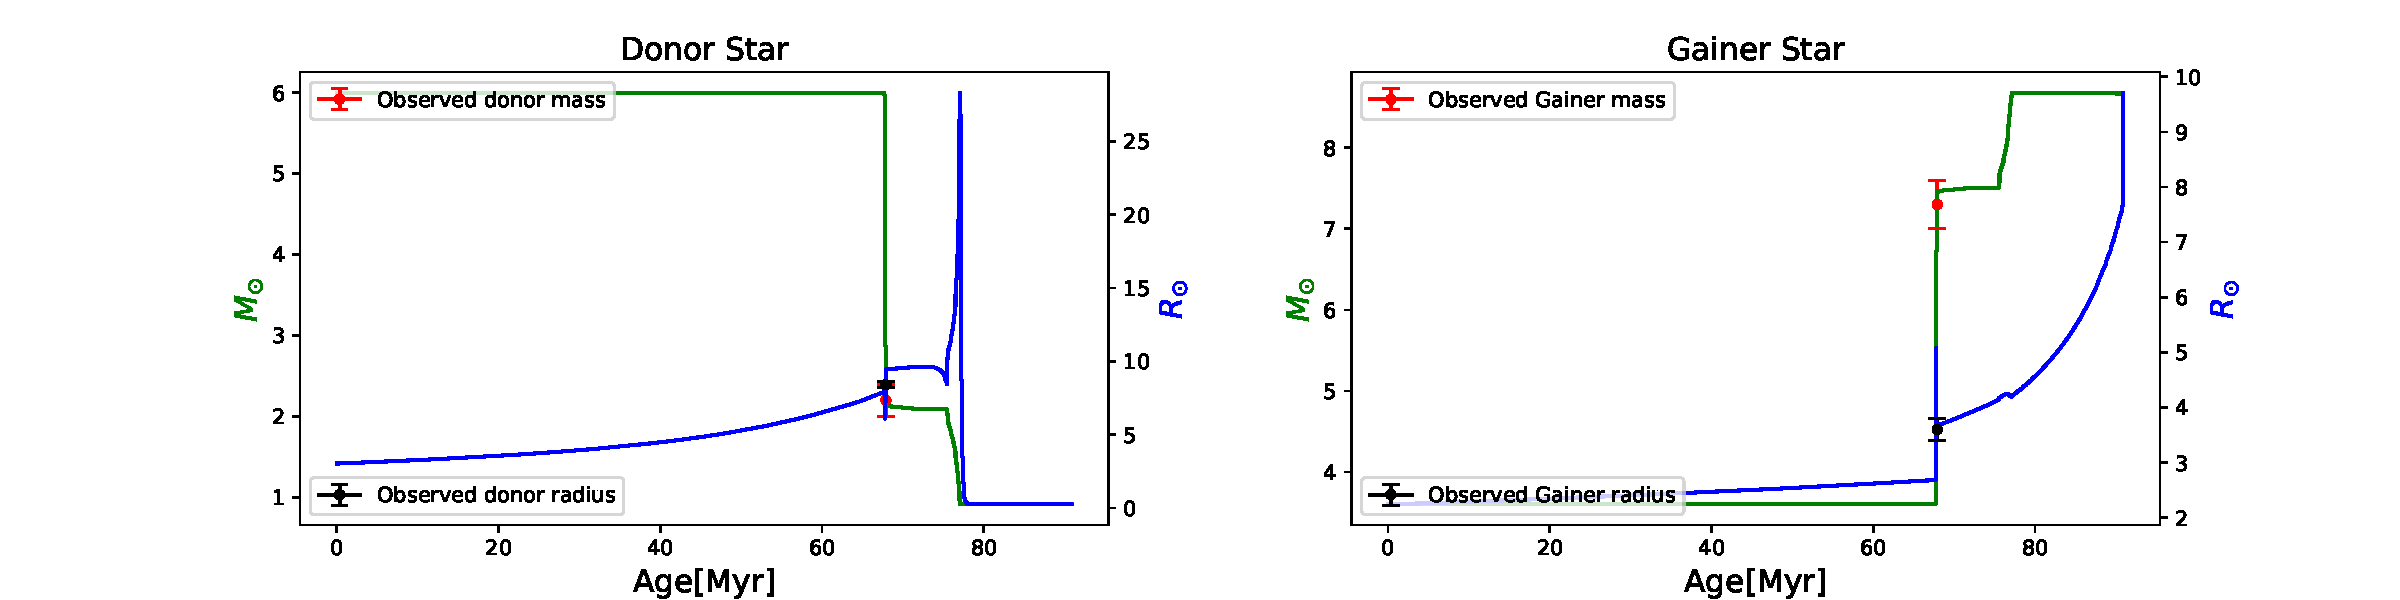
\includegraphics{dqvelmassradius.pdf}}
  \caption{Evolution of mass and radius of both binary components. On the left the figure shows the evolution of mass (green path) and radius (blue path) of the donor star also is plotted the current state of the donor component in red and black dots for mass and radius respectively. On the right the figure shows the evolution of mass (green path) and radius (blue path) of the gainer star also is plotted the current state of the gainer component in red and black dots for mass and radius respectively. Both stars are the components of DQ Velorum system.}
  \label{dqvel_evolution}
\end{figure*}


\subsection{Evolution of the dynamo number and long-to-short period over the age of the systems}
